\documentclass[10pt,conference,compsocconf]{IEEEtran}

\usepackage{hyperref}
\usepackage{graphicx}
\usepackage{booktabs} 

\begin{document}
\title{The Comfort Food Paradox - Milestone 2}

\author{
  Imane Benkamoun, Quirin Bitter, Sofia Taouhid\\
  \textit{Flavor Explorers}
}

\maketitle

\section{Project Goal}

Building on our first milestone, our goal is to deliver an interactive, scroll-driven data story answering the following question: \textbf{does pleasure come at the cost of health?} We want the visitor to scroll through a narrative that explains "comfort food" not as a moral failure but as chemistry. Some ingredients hit specific neuro-chemical pathways (for example, tyrosine and phenylalanine feeding dopamine or tryptophan feeding serotonin), so the foods we crave are not as random as we would think. We want them to arrive convinced that "tasty" and "healthy" are opposites and leave understanding that the relationship is far more nuanced, that their own weekly spending already reveals where they sit on the pleasure–health spectrum. 

The final product for now is a single-page scrolling website that walks the user through six chapters, each pairing a short narrative with one focused visualization. The story alternates between large-scale analysis and personal reflection, ending on an interactive tool that lets the user explore where their own favorite dishes land.

\section{What is already done}
Since Milestone 1:

\begin{itemize}
    \item We have built a Figma file with our desired final design and constructed a first skeleton of the website. This first draft is static compared to our final website that will be interactive.
    \item We have scaled and rebuilt the data pipeline. It now starts from the raw 62k Kaggle recipes, cleans and tokenizes each ingredient string, deduplicates recipes that the source dataset had repeated across categories, and runs a fuzzy match against FlavorDB's 1530 canonical ingredients. The result is 25\,009 unique recipes built from 9\,879 unique ingredients, of which 6\,311 (64\%) match FlavorDB and 3\,363 carry at least one mood-relevant compound drawn from our hand-curated mood mapping dataset. That mapping links 40 compounds onto 6 mood categories. Healthy scores are LLM-labelled on $[-1, 1]$, and mood scores are the summed weights of the mood-active compounds in each ingredient, traced through the FlavorDB chemistry chain. 
\end{itemize}

\section{Website Structure \& Figma Prototype}

Our desired design and interactive prototype is available at \url{https://mint-atom-61616656.figma.site/}. This Figma mockup serves as the visual blueprint for our project. It demonstrates our chosen color palette, typography, and UI layout while providing a clear preview of the scrollytelling transitions. By mapping out the visual journey in advance, we ensure the user experience feels cohesive and narrative-driven before full D3.js implementation. 

The storyboard contains the visual identity that we want for our website, which is heavily inspired by our desire to make health "fun", instead of it being a "clinical" topic, while at the same time, keeping a very minimal take on our website. The plots and data shown on the website do not correspond to the real data, but more as placeholders for our real data that is coming.


\section{Visualizations}

For now, here are the visualizations we will have in our website:

\begin{itemize}
    \item \textbf{Pleasure vs.\ Health Scatter (The Trade-Off Myth).} A 2D scatter with each point a recipe, $x$ = healthiness score (LLM-derived), $y$ = pleasure score (flavor complexity $\times$ mood-compound density).
    \item \textbf{Weekly Spending Bars (Your Weekly Reality).} A grouped bar chart (7 days $\times$ 2 categories: comfort vs.\ healthy spending share). Animated on scroll, with annotations for the Friday/Sunday peaks.
    \item \textbf{Cravings Donut (What We Actually Crave).} A donut chart showing the breakdown of dominant flavor profiles among comfort-labeled recipes (sweet, salty, fatty, umami, other). Click a slice to filter the scatter in V1.
    \item \textbf{Mood-Compound Spider (The Balance Breakdown).} Two/Three overlaid spider charts (comfort vs.\ healthy) on six axes: energy, serotonin precursors, magnesium, dopamine triggers, satiety, vitamins. Toggle between average profiles.
    \item \textbf{Interactive Balance Tool (Find Your Balance).} A drag-and-drop game where the user picks dishes and drops them on a plate. A live gauge shows the resulting balance score for healthiness and mood.
    \item \textbf{Ingredient Molecular Network (The Flavor Web).} A force-directed graph where nodes are ingredients and edges represent shared molecular compounds. This visualization justifies our chemical narrative, proving that ingredient pairings are driven by shared molecular profiles.
\end{itemize}

\begin{figure}[h]
    \centering
    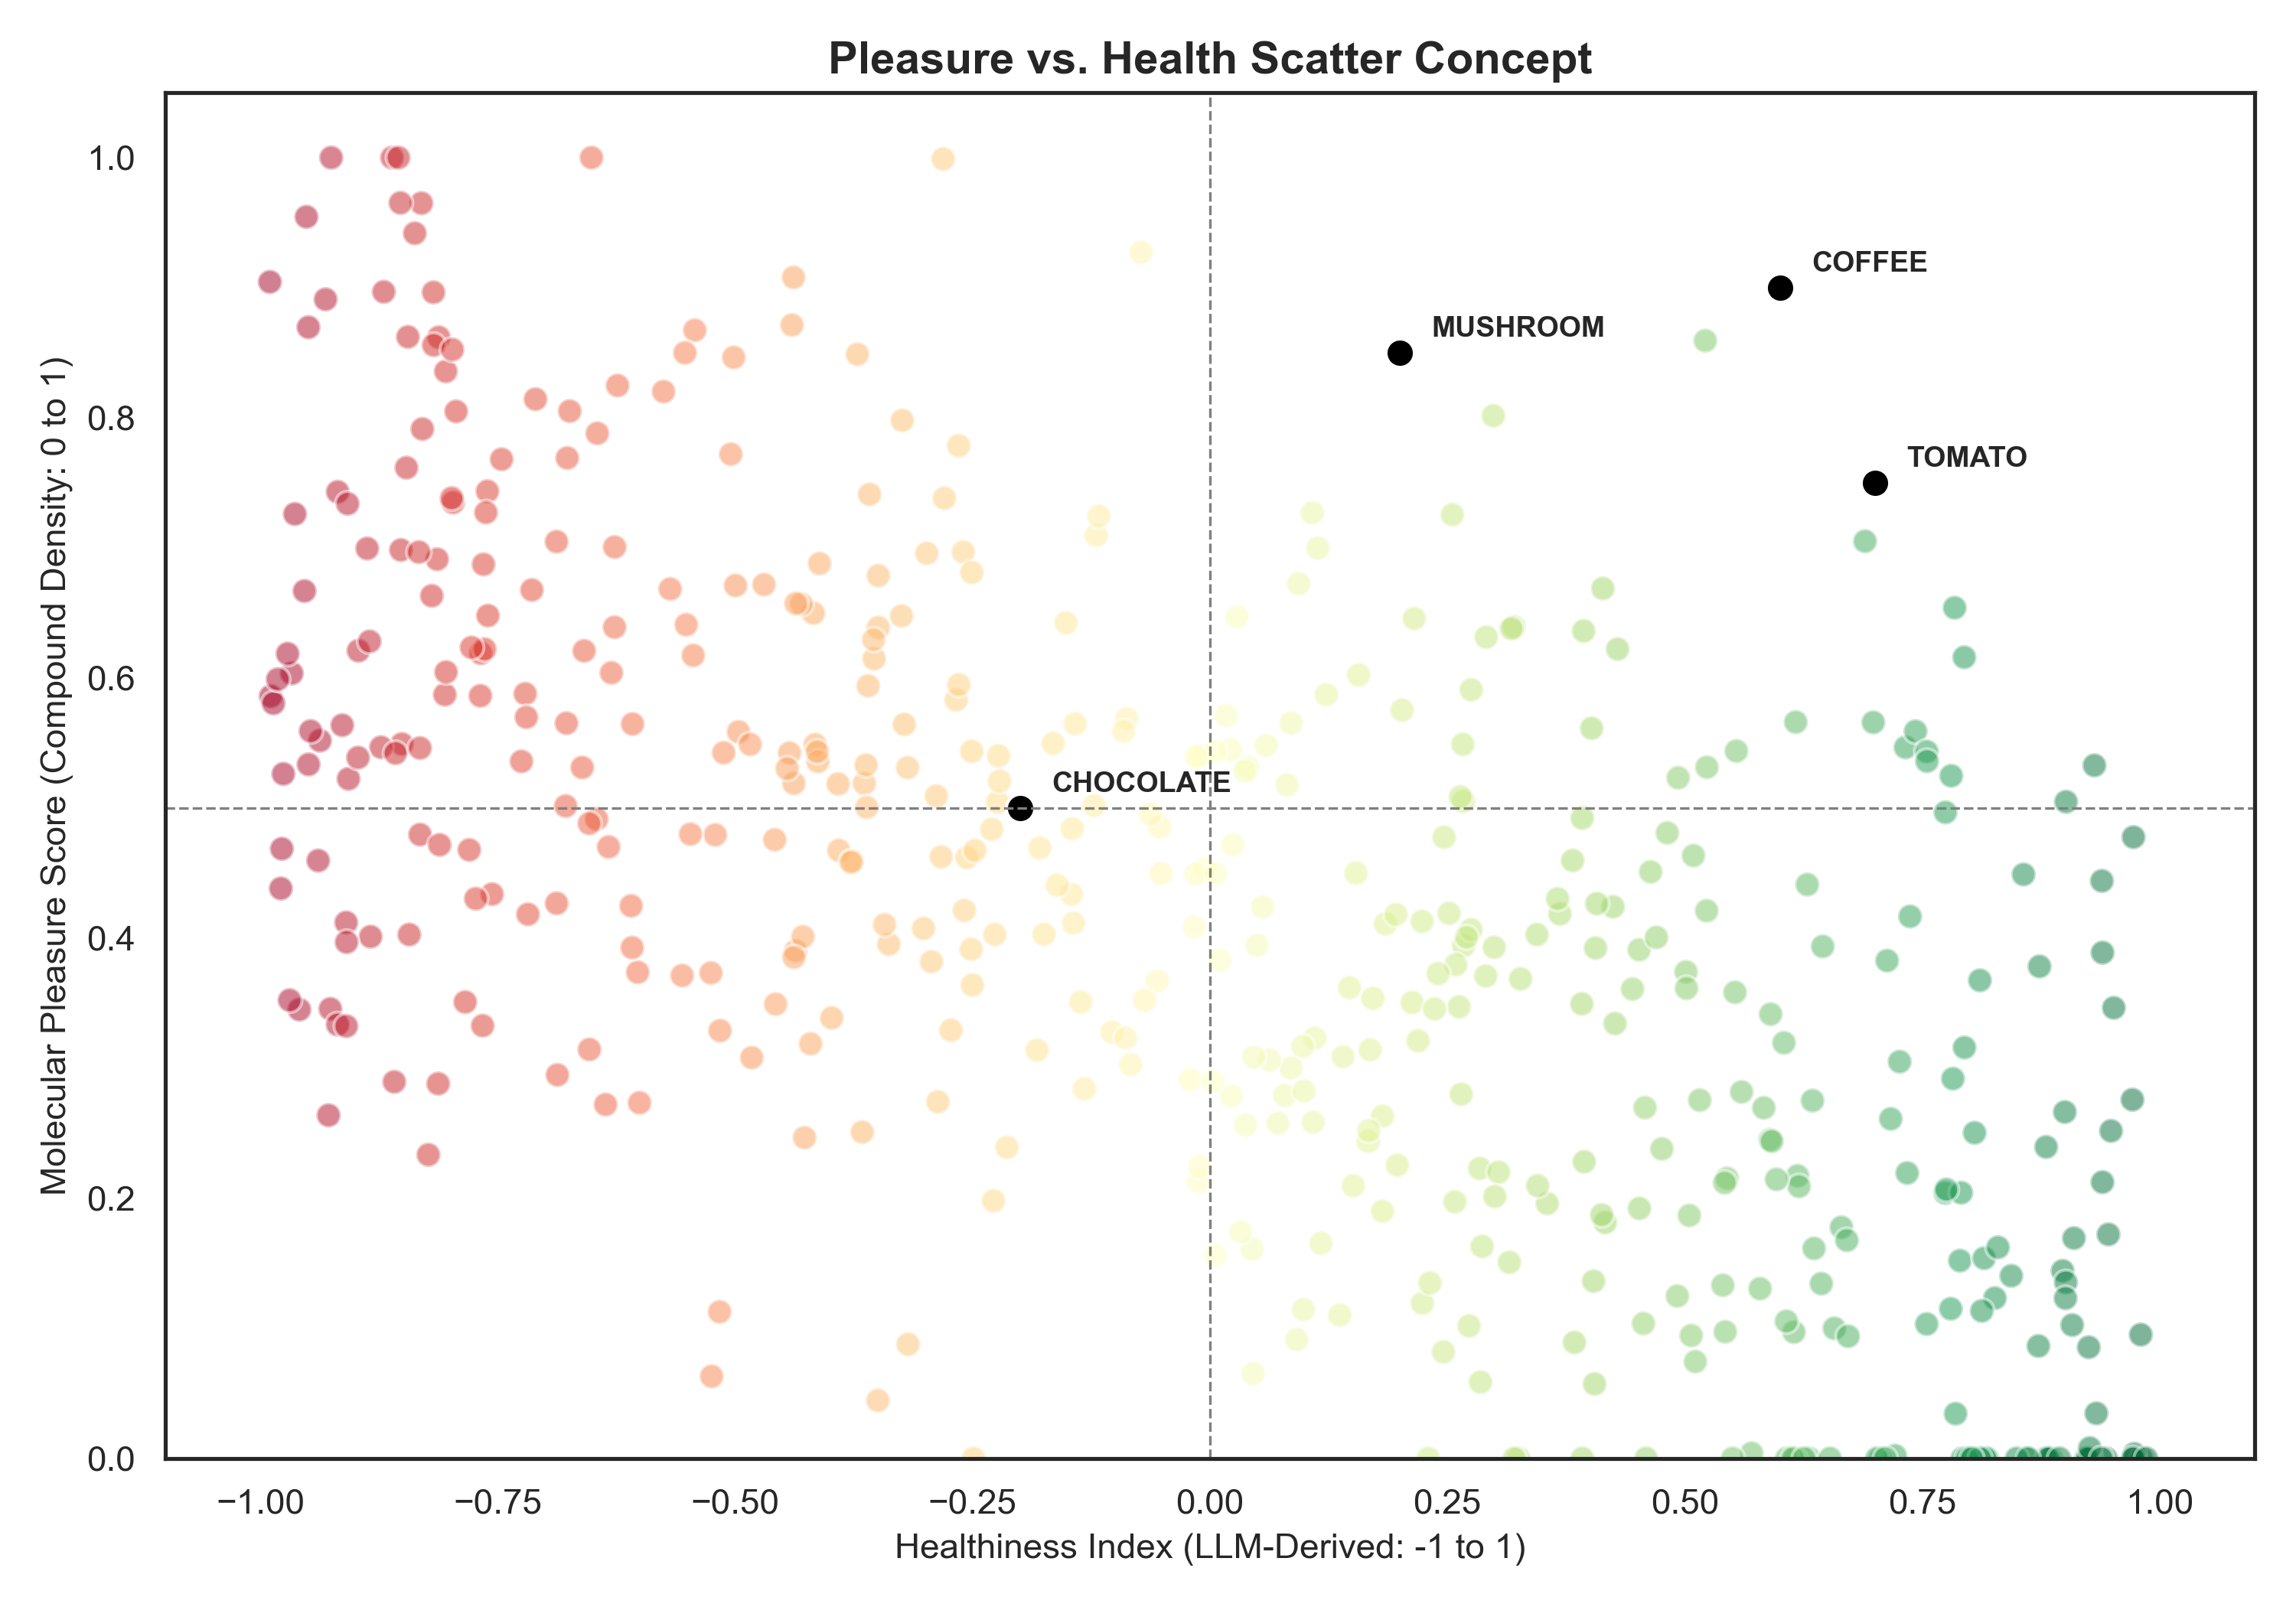
\includegraphics[width=\linewidth]{plots/scatter_plot_milestone2.png}
    \caption{Skelteon of the macro-scale distribution of 25,000 recipes. The x-axis represents the LLM-derived health score, while the y-axis reflects the molecular pleasure score derived from FlavorDB compound density.}
    \label{fig:scatter_plot}
\end{figure}

\begin{figure}[h]
    \centering
    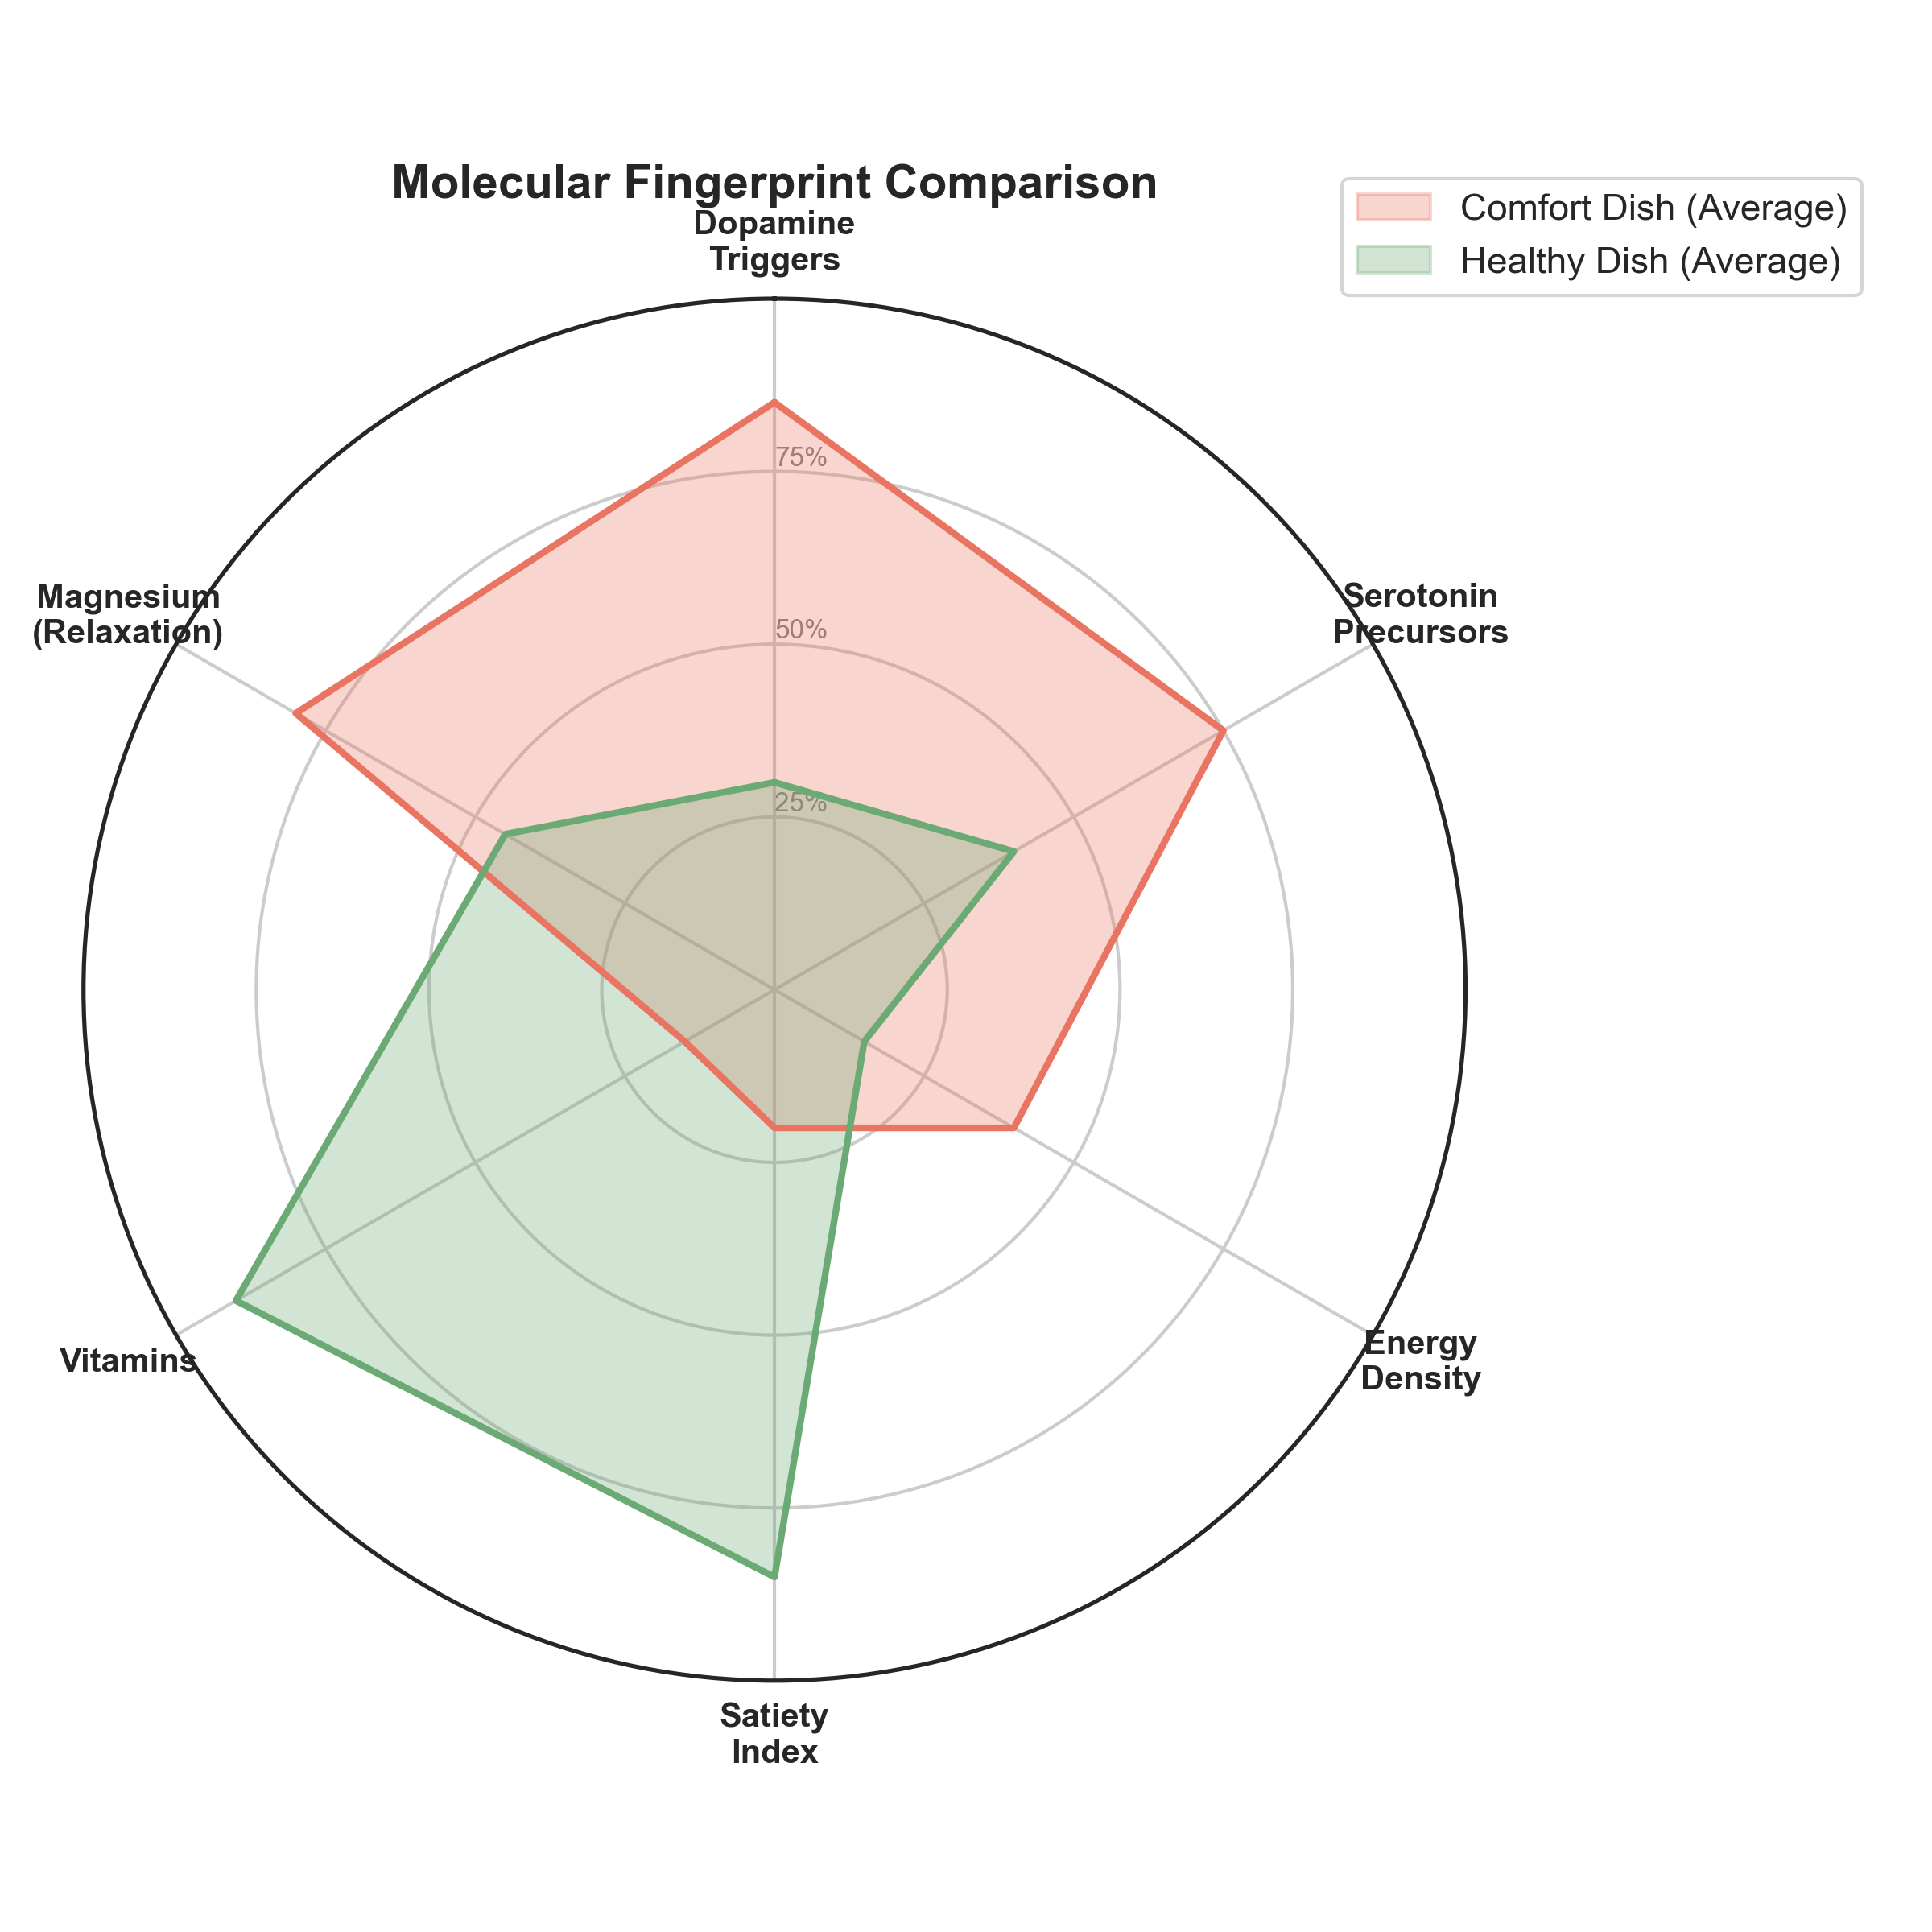
\includegraphics[width=0.9\linewidth]{plots/spider_chart_milestone2.png}
    \caption{Skeleton of the Molecular Fingerprint Comparison: A radar plot comparing the neuro-chemical profiles of a typical comfort dish vs. a healthy alternative across our six curated mood-active axes.}
    \label{fig:spider_chart}
\end{figure}

\begin{figure}[h]
    \centering
    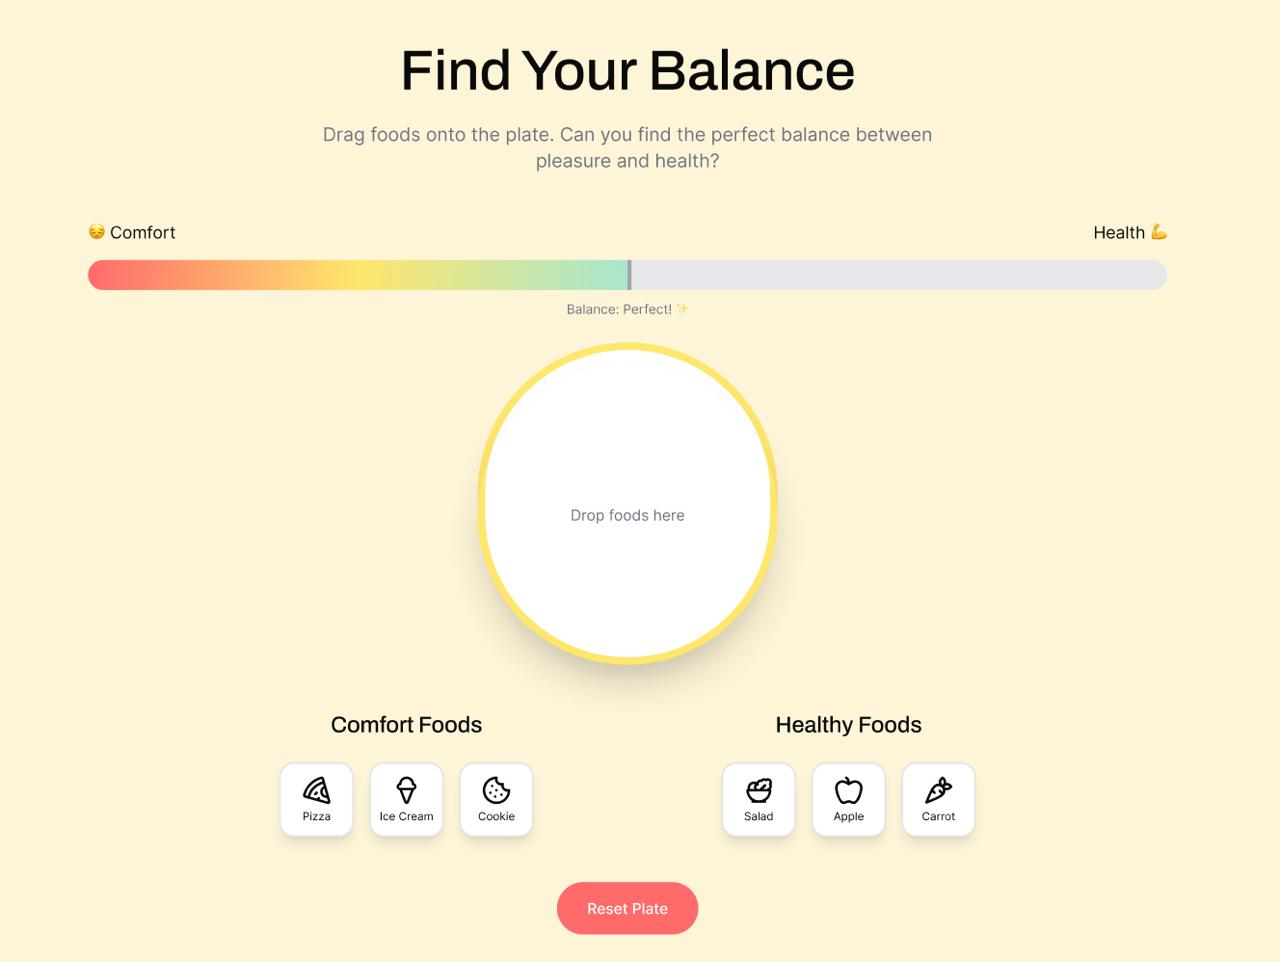
\includegraphics[width=0.9\linewidth]{plots/plate_game.jpg}
    \caption{Skeleton of the Interactive Balance Tool: A drag-and-drop game where the user picks dishes and drops them on a plate to see the resulting balance score between healthiness and mood.}
    \label{fig:spider_chart}
\end{figure}

\section{Tools \& Lectures Required}

\subsection*{Data Pipeline}
The data pipeline is built in Python with \texttt{pandas}. We used the custom regex-based ingredient tokenizer and the two-pass matcher against FlavorDB. Healthy-score labeling was done once via the Mistral API, which keeps the rest of the pipeline fully deterministic. This work draws on what we learned about data representation and preprocessing in the Data lecture 4.1 and will learn on tabular data handling from lecture 11.1.

\subsection*{Website \& Visualization}
The full visual design sketch (layout, typography, color palette, narrative flow) was built in Figma, giving us a clear visual target for Milestone 3 without getting stuck on implementation details. The website skeleton is built from scratch with HTML, CSS, and JavaScript on a vertical-scrolling system. We chose not to use a predefined framework so we keep full control over layout and transitions. \\
For the visualizations we are going to use the D3.js library. For now we added, mostly static, stub visualizations. For the final website we will create interactive visualization, where we present the user with updated respectively more detailed data on \textit{an interaction request}.\\
For the technical aspects we rely on our HTML/CSS/Javascript knowledge gained in the first five lectures and the homework readings, especially "Interactive Data Visualization for the Web" by Scott Muray. \\
For the design aspect we will refer to the perception principles from the 6th lecture and probably some general insights we hope to get from the 7th lecture.


\section{Extension Ideas}

\begin{itemize}
    \item \textbf{The "Chemical Twin" Recommender:} We intend to build a smart substitution engine. If a user inputs a high-pleasure/low-health dish (like a burger), the tool will use a nearest-neighbor algorithm to find its "chemical twin" (a recipe with a similar neuro-chemical profile but a significantly higher health score). 
    \item \textbf{Our Everyday Craving Clock:} Using the biological pathways of our 40 curated compounds, we can map ingredients to the human circadian rhythm. A circular heatmap would visualize which ingredients are "Morning Seekers" (Dopamine/Tyrosine for alertness) versus "Evening Soothers" (Serotonin/Melatonin precursors for sleep). This adds a temporal dimension to the Comfort Paradox, suggesting that our cravings change as our biological needs shift throughout the day. 
    \item \textbf{Expenditure Trajectories (The Long Game).} A multi-line chart, 1974--2024, with one line per major category (e.g.\ ready meals, fresh produce, sugary drinks). User can highlight a single line; recession years shown as vertical bands.
\end{itemize}

\end{document}